\documentclass{article}

\textwidth=6.5in
\textheight=8.5in
\voffset=-54pt
\oddsidemargin=0in
\evensidemargin=0in
\setlength{\parskip}{8pt}
\setlength{\parindent}{0pt}

\usepackage{amsmath, amssymb}
\usepackage{ifthen}

\usepackage[inline]{enumitem}
\setlist{topsep=0pt, parsep=8pt}

\usepackage[rgb,table]{xcolor}\convertcolorsUfalse
\usepackage{graphicx}

% change hyperref options
\PassOptionsToPackage{hyphens}{url}
\usepackage[bookmarks,colorlinks,linkcolor=black,citecolor=blue,pdfstartview=FitH,urlcolor=blue]{hyperref}
\hypersetup{pdfpagemode=UseNone}
\usepackage{bookmark}

\usepackage{graphicx}
\usepackage{multicol}
\usepackage{framed}
\usepackage{array}

\usepackage{icomma}

\usepackage{pifont}
\newenvironment{noanswer}{}{}
\newlist{altenumerate}{enumerate}{3}

\usepackage{soul}

\usepackage{pgfplots}
\pgfplotsset{compat=1.18}  
\pgfplotscreateplotcyclelist{mycolor}{black, blue, red, green!70!black, magenta, purple, cyan, orange }  
\pgfplotsset{
  disabledatascaling,
  cycle list=tikzcolor, 
  axis lines=middle,
  every axis plot/.style={no marks, thick},
  every axis/.style={
    enlarge x limits=false,
    enlarge y limits=auto,
    xlabel style={at={(current axis.right of origin)},anchor=west},
    ylabel style={at={(current axis.above origin)},anchor=south},
    % extra x and y ticks for asymptotes
    extra x tick style={grid=major, grid style={dashed,black}},
    extra y tick style={grid=major, grid style={dashed,black}},
    /pgf/number format/1000 sep={},
  },    
  tick label style = {font=\footnotesize, fill=\currentbgcolor, inner sep=0pt},    
  xticklabel shift=1pt,    
  scaled ticks=false,
  scaled y ticks=false,
  unbounded coords=jump,
  samples=101,
  minor tick length=0,
  scatter/classes={
    open={mark=*,draw=black,fill=white, mark size=2, thin},
    closed={mark=*,draw=black,fill=black, mark size=2, thin}
  },
  width=3in,
}
\pgfplotsset{open/.style={only marks, mark=*, fill=white, thin, mark size=2}}
\pgfplotsset{closed/.style={only marks, mark=*, draw=black, fill=black,
    thin, mark size=2}}
\pgfplotsset{labeled/.style={nodes near coords, only marks, mark=*, draw=black, fill=black, thin, mark size=2, point meta=explicit symbolic}}

\newcommand{\axes}[1][]{
  \begin{tikzpicture}
    \begin{axis}[xtick=\empty, ytick=\empty, ymin=-2, ymax=2,
      xmin=-4.25, xmax=4.25, #1]
    \end{axis}
  \end{tikzpicture}
}
\usepackage{tikz}
\usetikzlibrary{
  matrix,%
  % enables the snake paths
  decorations.pathmorphing,%
  % enables bigger arrows
  decorations.markings,%
  decorations.pathreplacing,%
  decorations.text,%
  calc,%
  patterns,%
  shapes.geometric,%
  arrows,
  decorations.shapes,
  positioning,
  plotmarks,
  intersections
}
\tikzset{>=latex} % sets default arrow type in tikz
\tikzset{font=\normalsize}
\tikzset{mark size=1.5pt, mark options=thin}
\tikzset{pin distance=4pt,
  every pin edge/.style={<-, thin, shorten <= -2pt}}

\interfootnotelinepenalty=10000
\renewcommand{\thefootnote}{(\arabic{footnote})}

\usepackage{multirow, bigdelim}

% change to \usepackage[sols]{handout} to see solutions
\usepackage{handout}

\newcommand\iscurrentenumi[1]{%
  \ifthenelse{\equal{#1}{\theenumi}}{}{#1}}
\setenumerate[1]{ref=\#\arabic*}
\setenumerate[2]{ref=\protect\iscurrentenumi{\theenumi}(\alph*)}
\newcommand\enumiiprefix[2]{%
  \ifthenelse{{\equal{#1}{\theenumi}}\AND{\equal{#2}{(\alph{enumii})}}}{}{}%
  \ifthenelse{{\equal{#1}{\theenumi}}\AND{\NOT{\equal{#2}{(\alph{enumii})}}}}{#2}{}%
  \ifthenelse{\equal{#1}{\theenumi}}{}{#1#2}%
}
\setenumerate[3]{ref=\protect\enumiiprefix{\theenumi}{(\alph{enumii})}\roman*}

\newlength{\tipmargin}
\makeatletter

\newdimen\SOUL@dimen %new
\def\SOUL@ulunderline#1{{%
    \setbox\z@\hbox{#1}%
    % \dimen@=\wd\z@
    \SOUL@dimen=\wd\z@ %new
    \dimen@i=\SOUL@uloverlap
    \advance\SOUL@dimen2\dimen@i %\dimen@ exchanged too
    \rlap{%
      \null
      \kern-\dimen@i
      % \SOUL@ulcolor{\SOUL@ulleaders\hskip\dimen@}%
      \SOUL@ulcolor{\SOUL@ulleaders\hskip\SOUL@dimen}% new
    }%
    \unhcopy\z@
  }}

\renewenvironment{framed}{
  \setlength{\tipmargin}{\textwidth-\linewidth}
  \advance\@totalleftmargin-\tipmargin
  \def\FrameCommand{\hspace{\tipmargin}\fbox}%
  \advance\linewidth\tipmargin
  \MakeFramed {\advance\hsize-\width \FrameRestore}%
}
{\endMakeFramed}

\makeatother

\newcommand{\related}[1]{%
\fcolorbox{black}{yellow}{%
  %\parbox[t]{12pt}{$\clubsuit$}%
  \parbox[t]{\linewidth-8pt}{\emph{Related problems:} #1}}}

\renewcommand{\answer}[1]{#1}

\definecolor{purple}{rgb}{0.5,0,1.0}
\definecolor{hotpink}{rgb}{1, 0, 0.5}
\definecolor{darkorange}{rgb}{1, 0.4, 0}

\definecolor{skyblue}{rgb}{0, 0.5, 1}

\newcounter{imagecounter}
\newcounter{columncounter}
\newenvironment{imagetable}[3][]{%
  \setcounter{imagecounter}{0}
  \setcounter{columncounter}{#2}
  \addtocounter{columncounter}{-1}
  \newcolumntype{i}{>{\raisebox{-1ex-\height}{\makebox[1em]{\hfill\stepcounter{imagecounter}(#3{imagecounter})}}\hspace{4pt}\begin{minipage}[t]{\linewidth/#2-1em-\tabcolsep*3}\arraybackslash\vspace{0pt}}l<{\end{minipage}}}
\begin{tabular}{i*{\value{columncounter}}{#1i}}}
{\end{tabular}}  

\newcommand{\goal}[1]{\textbf{\textcolor{skyblue}{#1}}}
\newcommand{\indvar}[1]{\textbf{\textcolor{hotpink}{#1}}}
\newcommand{\concaveup}{\raisebox{-1pt}{\tikz[x=0.075cm,y=0.075cm] \draw (-2, 4) parabola bend (0, 0) (2, 4);}}

\usepackage{amsthm}

% make URLs print in the same font
\usepackage{url}
\urlstyle{same}

\usepackage{pifont}
\def\exend{\hfill\ding{118}}

%\makeatletter\@addtoreset{equation}{section}\makeatother
%\renewcommand{\theequation}{\arabic{section}.\arabic{equation}}

\newtheoremstyle{theorem}% name
{8pt}%      Space above
{0pt}%      Space below
{\itshape}%         Body font
{}%         Indent amount (empty = no indent, \parindent = para indent)
{\bfseries}% Thm head font
{.}%        Punctuation after thm head
{.5em}%     Space after thm head: " " = normal interword space;
                                %       \newline = linebreak
{}%         Thm head spec (can be left empty, meaning `normal')

\theoremstyle{theorem}

\let\Theorem\undefined
\newtheorem{Theorem}[equation]{Theorem}
\let\Definition\undefined
\newtheorem{Definition}[equation]{Definition}
\let\Summary\undefined
\newtheorem{Summary}[equation]{Summary}
\let\Conjecture\undefined
\newtheorem{Conjecture}[equation]{Conjecture}
\let\Fact\undefined
\newtheorem{Fact}[equation]{Fact}

\renewcommand{\thesubsection}{\arabic{subsection}}
\makeatletter
\def\@seccntformat#1{\@ifundefined{#1@cntformat}%
   {\csname the#1\endcsname\quad}%       default
   {\csname #1@cntformat\endcsname}}%    enable individual control
\newcommand\section@cntformat{}
\makeatother

  \usepackage{exam}

\usepackage{fancyhdr}
\lhead{\textcolor{white}{This content is protected and may not be shared, uploaded, or distributed.}}
\rhead{}
\rfoot{\vspace*{\fill}\footnotesize\textcopyright{} \emph{Harvard Math Ma}}
\renewcommand{\headrulewidth}{0pt}
\pagestyle{fancy}
\begin{document}

  \title{Exam 1, Practice 3}

\instructions{instructions.tex}{}

\listofproblems

\begin{enumerate}
\item \label{fall2012-1a-midterm1-2a} \points{11} 

  You leave from Boston on Saturday at 11 am for a trip back and forth
  along a north-south railroad line to see the fall leaves changing color.
  Here is a graph of your \textbf{velocity}, in miles per hour, $t$ hours
  after noon.  Here, $v(t) > 0$ represents traveling north and $v(t) <0$
  traveling south.

  \begin{center}
    \begin{tikzpicture}
      \begin{axis}[ytick={-100, -80, ..., 80}, width=4in, height=2.5in, 
        xlabel=$t$, ylabel=velocity]
        \addplot+[domain=0:4] {-100 + (864*(19/6 - 7*x + (9*x^2)/2
          - (2*x^3)/3))/25}; 
      \end{axis}
    \end{tikzpicture}
  \end{center}

  For each of the following, circle one answer and briefly explain your
  reasoning.
  \begin{enumerate}
  \item \label{fall2012-1a-midterm1-2a-i}
    \begin{problem}[\vfill]
      At time $t = 1$, your velocity is: \qquad \maybecircle[0=1]{positive}
      \qquad \maybecircle[1=1]{negative} \qquad \maybecircle[0=1]{zero} \qquad
      \maybecircle[0=1]{not enough info}

      \probonly{\textbf{Reasoning:}}
    \end{problem}

    \begin{solution}
      The graph shows that $v(1) \approx -100$. The key here is to remember that the graph shows \emph{velocity}, not position. \answeronly{negative}
    \end{solution}

  \item
    \begin{problem}[\vfill]
      At time $t = 1$, you are traveling: \qquad \maybecircle[0=1]{north}
      \qquad \maybecircle[1=1]{south} \qquad \maybecircle[0=1]{not enough
        info}

      \probonly{\textbf{Reasoning:}}
    \end{problem}

    \begin{solution}
      We're told that negative velocity indicates traveling south, and we saw in \ref{fall2012-1a-midterm1-2a-i} that our velocity at $t=1$ is negative. \answeronly{south}
    \end{solution}

  \item
    \begin{problem}[\vfill]
      At time $t = 3$, your position is: \qquad \maybecircle[0=1]{north of
        Boston} \qquad \maybecircle[0=1]{south of Boston} \qquad
      \maybecircle[1=1]{not enough info}

      \probonly{\textbf{Reasoning:}}
    \end{problem}

    \begin{solution}
      The trip started at 11 am, but the velocity graph only says what happens between noon and 4 pm. Since we have no idea what happened between 11 am and noon, we have no idea where we were at noon, so we can't figure out where we were at 4 pm. \answeronly{not enough info}
    \end{solution}    

  \item \label{fall2012-1a-midterm1-2a-accel}
    \begin{problem}[\vfill\newpage]
      At time $t = 2$, your acceleration is: \qquad
      \maybecircle[1=1]{positive} \qquad \maybecircle[0=1]{negative} \qquad
      \maybecircle[0=1]{zero} \qquad \maybecircle[0=1]{not enough info}

      \probonly{\textbf{Reasoning:}}
    \end{problem}

    \begin{solution}
      Since acceleration is the derivative of velocity, this asks about the sign of $v'(2)$. We can visualize $v'(2)$ as the slope of the tangent line at $t=2$, which is positive. \answeronly{positive}
    \end{solution}

  \end{enumerate}

  \begin{problemonly}
    \begin{framed}
      \emph{Continued from previous page}
    \end{framed}
  \end{problemonly}

  \begin{enumerate}[resume]
  \item % added 2023
    \begin{problem}[\newpage]
      Sketch a graph of your acceleration $t$ hours after noon. 
    \end{problem}

    \begin{solution}
      Acceleration is the derivative of velocity, so we sketch the derivative of the given graph. 
      \begin{center}
        \answer{
          \begin{tikzpicture}
            \begin{axis}[ytick=\empty, width=4in, height=2.5in, 
              xlabel=$t$, ylabel=acceleration]
              \addplot+[domain=0:4] {(864*(-7 + 9*x - 2*x^2))/25}; 
            \end{axis}
          \end{tikzpicture}
        }
      \end{center}      
    \end{solution}

    \begin{grading}
      The key properties we're looking for:
      \begin{itemize}
      \item The acceleration is positive on $(1, 3.5)$ and negative otherwise.
      \item The acceleration is increasing on $(0, \approx 2.2)$ and decreasing otherwise. 
      \end{itemize}
    \end{grading}

  \end{enumerate}

\item \label{fall2019-midterm-practice1-6a-modified} \points{12} 

  Consider the function $f(x)= \displaystyle\frac{x}{3x+1} $.
  \begin{enumerate} 
  \item \label{fall2019-midterm-practice1-6a-modified-deriv}
    \begin{problem}[\vfill]
      Use the definition of the derivative to calculate $f'(3)$. Show all your work.
    \end{problem}

    \begin{solution}
      \begin{align*}
        f'(3) &= \lim_{h \to 0}\frac{f(3+h)-f(3)}{h} \\
        &= \lim_{h \to 0} \frac{\dfrac{3 + h}{3 (3 + h) + 1} - \dfrac{3}{10}}{h} \\
        &= \lim_{h \to 0} \frac{\dfrac{3 + h}{10 + 3h} - \dfrac{3}{10}}{h} \\
        &= \lim_{h \to 0} \frac{\quad \dfrac{(3 + h) 10 - 3 (10 + 3h)}{(10 + 3h) 10} \quad}{h} \\
        &= \lim_{h \to 0} \frac{30 + 10h - 30 - 9h}{h (10 + 3h) 10 } \\
        &= \lim_{h \to 0} \frac{h}{h(10 + 3h) 10} \\
        \intertext{When we take the limit as $h \to 0$, we're looking only at $h \neq 0$, so we can cancel the $\frac{h}{h}$:} % 
        &= \lim_{h \to 0} \frac{1}{(10 + 3h) 10} \\
        \intertext{Now that there's no $h$ in the denominator, we can just plug in $h = 0$ to evaluate the limit:}%
        &= \frac{1}{10^2} \\
        &= \boxed{\frac{1}{100}}
      \end{align*}
    \end{solution}

  \item
    \begin{problem}[\nstretch{0.4}]
      Find the equation of line tangent to $y = \dfrac{x}{3x + 1}$ at $x=3$.
    \end{problem}

    \begin{solution}
      The tangent line at $x=3$ passes through $(3, f(3))= \left(3, \frac{3}{10} \right)$. The slope of the tangent line is $f'(3)=\frac{1}{100}$. So, the equation of the tangent line is $\boxed{y - \frac{3}{10} = \frac{1}{100} (x - 3)}$.
    \end{solution}

  \item % added 2023 by Janet

    \begin{problem}
      Let $g(x) = \dfrac{x (x - 1)}{(3x + 1) (x - 1)}$. Which one of the following is the graph of $g$? Explain briefly. (Hint: Think about how $g$ relates to $f$ and what your answer to \ref{fall2019-midterm-practice1-6a-modified-deriv} tells you.)
    \end{problem}

    \begin{imagetable}{2}{\Alph}
      \begin{tikzpicture}
        \begin{axis}[width=2.5in, ymin=-0.33, ymax=1, ytick=\empty, xtick={-3, -2, -1, 1, 2, 3}]
          \addplot+[domain=-4:4, restrict y to domain=-2:2]{x/(3*x+1)}; 
        \end{axis}
      \end{tikzpicture} &
      \begin{tikzpicture}
        \begin{axis}[width=2.5in, ymin=-0.33, ymax=1, ytick=\empty, xtick={-3, -2, -1, 1, 2, 3}]
          \addplot+[domain=-4:4, restrict y to domain=-2:2]{2/3-x/(3*x+1)}; 
        \end{axis}
      \end{tikzpicture} \vspace{24pt} \\
      \begin{tikzpicture}
        \begin{axis}[width=2.5in, ymin=-0.33, ymax=1, ytick=\empty, xtick={-3, -2, -1, 1, 2, 3}]
          \addplot+[domain=-4:4, restrict y to domain=-2:2]{x/(3*x+1)};
          \addplot+[open] coordinates { (1, 1/4)}; 
        \end{axis}
      \end{tikzpicture} &
      \begin{tikzpicture}
        \begin{axis}[width=2.5in, ymin=-0.33, ymax=1, ytick=\empty, xtick={-3, -2, -1, 1, 2, 3}]
          \addplot+[domain=-4:4, restrict y to domain=-2:2]{2/3-x/(3*x+1)};
          \addplot+[open] coordinates { (1, 5/12)}; 
        \end{axis}
      \end{tikzpicture} 
    \end{imagetable}

    \begin{solution}
      $g(x)$ is undefined when $x = 1$, so we can eliminate choices A and B. When $x \neq 1$, $\dfrac{x - 1}{x - 1} = 1$, so $g(x) = \dfrac{x}{3x + 1} = f(x)$. Therefore, $g$ is identical to $f$ except that it's undefined at $x = 1$. We calculated that $f'(3) > 0$, so $f$ is increasing at 3. Therefore, $g$ should also be increasing at 3, so the correct graph must be \fbox{C}.
    \end{solution}

    \pspace{\vfill}

  \item
    \begin{problem}[\vfill]
      If $h(x) = 2x + 1$, find $f(h(x))$; please simplify your answer. (Remember that $f(x) = \dfrac{x}{3x + 1}$.) 
    \end{problem}

    \begin{solution}
      Since $h(x) = 2x + 1$, we have
      \begin{align*}
        f(h(x)) &= f(2x + 1) \\
        &= \frac{2x + 1}{3 (2x + 1) + 1} \\
        &= \boxed{\frac{2x + 1}{6x + 4}}
      \end{align*}
      If this is confusing, it may help to think about it like this: since $f(x) = \dfrac{x}{3x + 1}$, $f(\diamondsuit) = \dfrac{\diamondsuit}{3 \diamondsuit + 1}$. When we do $f(2x + 1)$, we're replacing $\diamondsuit$ by $2x + 1$. 
    \end{solution}
  \end{enumerate} 

  \pspace{\newpage}

\item \label{fall2019-midterm-practice2-7} \points{14} 

  Tim the beaver is standing on the north (unforested) bank of a river. There are trees all along the south side of the river, so Tim would like to cross the river to harvest a tree for his dam home. The river is 100 meters wide, and Tim's dam is in the middle of the river 500 meters downstream. Suppose Tim can swim 4 kilometers per hour while pulling a tree and 8 kilometers per hour without a tree. 

  Suppose Tim swims to the opposite shore $x$ meters downstream to harvest a tree. He swims in a straight line from his current position to the tree and then in a straight line from the tree to his dam.

  \begin{minipage}{0.6\textwidth}
    \begin{tikzpicture}
      \draw (-6, 3) -- (3, 3);%
      \draw (-6, 0) -- (3, 0);%
      \draw [thick, dotted] (2, 3) -- (2, 0);%
      \fill (2, 3) circle (2 pt) node[above] {Tim};%
      \fill (0, 0) circle (2 pt) node[below] {Tree};%
      \fill (-5, 1.5) circle (2 pt) node[above] {dam};%
      \draw [decorate, decoration={brace, amplitude=8pt}] (.0, 0) -- node[above, yshift=8pt]{$x$} (2, 0.0);%
      \draw [decorate, decoration={brace, amplitude=8pt}] (-5 , 3) -- node[above, yshift=8pt] {500} (2, 3);%
    \end{tikzpicture}
  \end{minipage}
  \begin{minipage}{0.3\textwidth}
    
\includegraphics[scale=0.5]{images/tim}
  \end{minipage}

  \solonly{\related{{{\#5}} on \href{https://people.math.harvard.edu/~jjchen/mathma/docs/worksheets/worksheet06-sols.html}{the worksheet ``Function Composition, Modeling with Functions''}; \ref{fall2015-1a-gateway-overview-24}}}

  \begin{enumerate}
  \item
    \begin{problem}[\vfill\newpage]
       Find the total distance Tim travels to get the tree and bring it to his dam as a function of $x$.
    \end{problem}

    \begin{solution}
      We'll use the same general strategy as in {{\#3}} on \href{https://people.math.harvard.edu/~jjchen/mathma/docs/worksheets/worksheet06-sols.html}{the worksheet ``Function Composition, Modeling with Functions''}: 

      \begin{noanswer}
        \begin{enumerate}[label=\arabic*.]
        \item \hl{\textbf{Understand the Problem.}}

          \begin{itemize}
          \item \hl{\textbf{Goal:}} Express \goal{total distance $d$} in terms of \indvar{$x$}.

          \item Drawing \textbf{a couple of very different examples} is a great way to get a feel for the situation.
            \begin{center}
              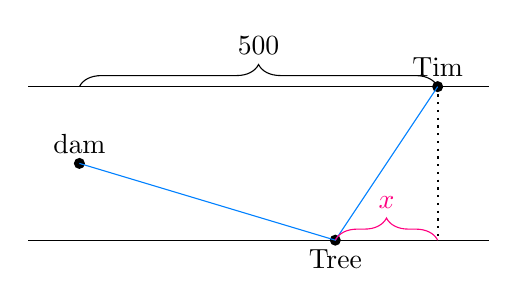
\begin{tikzpicture}[x=0.65cm, y=0.65cm]
                \draw (-6, 3) -- (3, 3);%
                \draw (-6, 0) -- (3, 0);%
                \draw [thick, dotted] (2, 3) -- (2, 0);%
                \fill (2, 3) circle (2 pt) node[above] {Tim};%
                \fill (0, 0) circle (2 pt) node[below] {Tree};%
                \fill (-5, 1.5) circle (2 pt) node[above] {dam};%
                \draw [decorate, decoration={brace, amplitude=8pt}] (-5 , 3) -- node[above, yshift=8pt] {500} (2, 3);%
                \draw[skyblue] (2, 3) -- (0, 0) -- (-5, 1.5);%
                \draw [decorate, decoration={brace, amplitude=8pt}, hotpink] (.0, 0) -- node[above, yshift=8pt]{$x$} (2, 0.0);%
              \end{tikzpicture}
              \hspace{0.4in}
              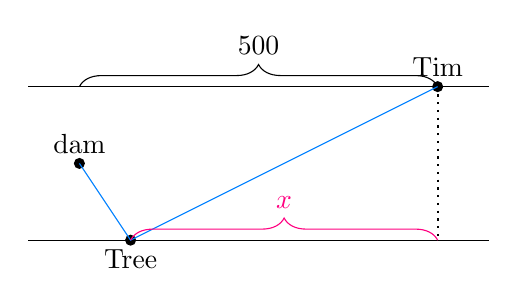
\begin{tikzpicture}[x=0.65cm, y=0.65cm]
                \draw (-6, 3) -- (3, 3);%
                \draw (-6, 0) -- (3, 0);%
                \draw [thick, dotted] (2, 3) -- (2, 0);%
                \fill (2, 3) circle (2 pt) node[above] {Tim};%
                \fill (-4, 0) circle (2 pt) node[below] {Tree};%
                \fill (-5, 1.5) circle (2 pt) node[above] {dam};%
                \draw [decorate, decoration={brace, amplitude=8pt}] (-5 , 3) -- node[above, yshift=8pt] {500} (2, 3);%
                \draw[skyblue] (2, 3) -- (-4, 0) -- (-5, 1.5);%
                \draw [decorate, decoration={brace, amplitude=8pt}, hotpink] (-4, 0) -- node[above, yshift=8pt]{$x$} (2, 0.0);%
              \end{tikzpicture}
            \end{center}
          \end{itemize}

        \item Since our goal is the \goal{total distance $d$}, let's \hl{\textbf{write a formula}} for it, \hl{\textbf{defining any variables we use}}. Here, we'll define variables by labeling them in our picture:
          \begin{center}
            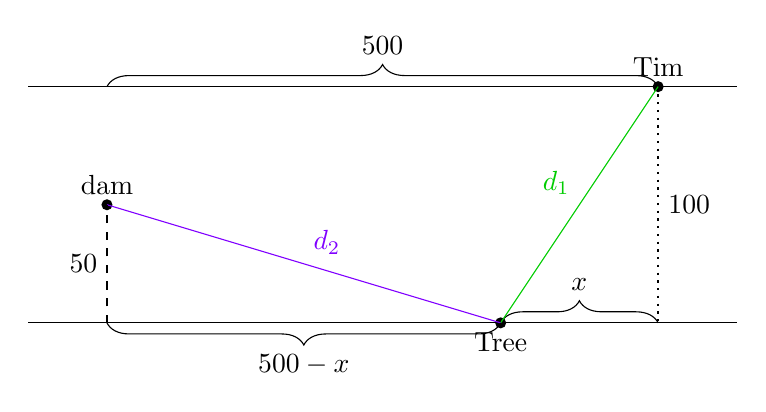
\begin{tikzpicture}
              \draw (-6, 3) -- (3, 3); %
              \draw (-6, 0) -- (3, 0); %
              \draw [thick, dotted] (2, 3) -- node[right]{100} (2, 0); %
              \fill (2, 3) circle (2 pt) node[above] {Tim}; %
              \fill (0, 0) circle (2 pt) node[below] {Tree}; %
              \fill (-5, 1.5) circle (2 pt) node[above] {dam}; %
              \draw [decorate, decoration={brace, amplitude=8pt}] (.0, 0) -- node[above, yshift=8pt]{$x$} (2, 0.0);%
              \draw [decorate, decoration={brace, amplitude=8pt}] (-5 , 3) -- node[above, yshift=8pt] {500} (2, 3);%
              \draw[green!80!black] (2, 3) -- node[anchor=south east]{$d_1$} (0, 0);%
              \draw[purple] (0, 0) -- node[anchor=south west]{$d_2$} (-5, 1.5);%
              \draw[dashed] (-5, 0) -- node[left]{50} (-5, 1.5);%
              \draw [decorate, decoration={brace, amplitude=8pt}] (0, 0) -- node[below, yshift=-8pt]{$500 - x$} (-5, 0);%
            \end{tikzpicture}
          \end{center}
          \[ \text{\textbf{Formula: }} \goal{total distance $d$} = d_1 + d_2 \]

        \item Now, we need to \hl{\textbf{relate the variables we've used}} ($d_1$ and $d_2$) so that we can get everything in terms of the desired variable (\indvar{$x$}). To do this, we must \hl{\textbf{use something else we know about the situation}}. Here, we can use the Pythagorean Theorem on the two right triangles in the picture, which gives
          \begin{itemize}
          \item $100^2 + x^2 = d_1^2$, so $d_1 = \sqrt{100^2 + x^2}$.
          \item $50^2 + (500 - x)^2 = d_2^2$, so $d_2 = \sqrt{50^2 + (500 - x)^2}$.
          \end{itemize}
          Plugging these into our formula for distance, $\goal{$d$} = \boxed{\sqrt{100^2 + x^2} + \sqrt{50^2 + (500 - x)^2}}$ meters.
        \end{enumerate}
      \end{noanswer} \answeronly{$\displaystyle \sqrt{100^2 + x^2} + \sqrt{50^2 + (500 - x)^2}$} 
    \end{solution}

  \item
    \begin{problem}[\nstretch{0.8}]
      Find the total time Tim travels as a function of $x$.
    \end{problem}

    \begin{solution}

      \hl{\textbf{Goal:}} Express \goal{total time $T$} in terms of $x$.

      Using the picture from the previous part, 
      \begin{align*}
        \goal{$T$} &= \text{time to swim $d_1$} + \text{time to swim $d_2$} \\
        \intertext{Since $\text{distance} = \text{rate} \cdot \text{time}$, $\text{time} = \dfrac{\text{distance}}{\text{rate}}$, so we can rewrite our formula for \goal{$T$} as:}
        &= \dfrac{d_1}{\text{swimming speed without tree}} + \dfrac{d_2}{\text{swimming speed with tree}} \\
        \intertext{Since $d_1, d_2$ are in meters, we need to express the speeds in meters per hour:} % 
        &= \boxed{\frac{\sqrt{100^2+x^2}}{8000}+\frac{\sqrt{50^2 + (500-x)^2}}{4000}}  \text{ hours}
      \end{align*}
    \end{solution}

  \end{enumerate}

\item \label{fall2015-1a-m2practice4-4} \points{5} 

  Ron has decided to start a business making jam.  Suppose $C(p)$ is the
  cost, in dollars, for Ron to make $p$ ounces of jam.

  \begin{enumerate}
  \item
    \begin{problem}[\vfill]
      What are the units of $\dfrac{dC}{dp}$?  
    \end{problem}

    \begin{solution} % Jason Bland
      Since $C$ is in dollars and $p$ is in ounces, the units of $\frac{dC}{dp}$ are \fbox{dollars per ounce}.
    \end{solution}

  \item \label{interpret-derivative-ron-jam-choose}
    \begin{problem}[\vfill]
      Which of the following two is the more reasonable value of $\dfrac{dC}{dp}$ when $p = 30$? Explain.
      \[ \frac{1}{2} \hspace{1in} -\frac{1}{2}\]
    \end{problem}

    \begin{solution}
      $C(p)$ should be an increasing function: the more ounces of jam Ron makes, the more the total cost should be. Therefore, $\frac{dC}{dp}$ should be positive, so $\boxed{\frac{1}{2}}$ is the more reasonable value.
    \end{solution}

  \item
    \begin{problem}[\vfill\newpage]
      Suppose that, when $p = 30$, $\dfrac{dC}{dp}$ is the value you chose in \ref{interpret-derivative-ron-jam-choose}. Do you have enough information to make a good estimate of how much it costs for Ron to make 30 ounces of jam? If so, do so; if not, explain why not.
    \end{problem}

    \begin{solution}
      We're assuming $C'(30) = \frac{1}{2}$, but this is \fbox{not enough information} to estimate $C(30)$. Graphically, knowing $C'(30)$ tells us the slope of the graph of $C(p)$ at $p = 30$, but it doesn't tell us anything about how high the graph is at that point.
    \end{solution}

  \end{enumerate}

\item  \points{13} 

  Let $g(x) = \sqrt{x - 1} - 2$.

  \begin{enumerate}
  \item
    \begin{problem}[\vfill]
      Sketch the graph of $g$. Make sure important features such as the domain, range, and intercepts are clear. 
    \end{problem}

    \begin{solution}
      We can get this graph by starting with $y = \sqrt{x}$ and shifting it 1 unit right and 2 units down. That makes $(1, -2)$ a point on the graph. The graph now has a new $x$-intercept; to find it, we solve
      \begin{align*}
        \sqrt{x - 1} - 2 &= 0 \\
        \sqrt{x - 1} &= 2 \\
        x - 1 &= 4 \\
        x &= 5
      \end{align*}
      So, here's a labeled graph:
      \begin{center}
        \answer{
          \begin{tikzpicture}
            \begin{axis}[xtick={1, 5}, ytick={-2}, xmin=0]
              \addplot+[domain=1:2] {sqrt(x - 1) - 2}; %
              \addplot+[domain=2:12] {sqrt(x - 1) - 2}; %
              \addplot+[closed] coordinates { (1, -2) } node[below]{$(1, -2)$}; % 
            \end{axis}
          \end{tikzpicture}
        }
      \end{center}
    \end{solution}

  \end{enumerate}

  Suppose $f$ is a function with the following properties:
  \begin{itemize}[nosep]
  \item $f$ has domain $[1, \infty)$ and is continuous on its domain.
  \item $f'(x) = g(x)$ (where $g(x)$ is still $\sqrt{x - 1} - 2$).
  \item $f(1) = 0$.
  \end{itemize}

  \begin{enumerate}[resume]
  \item
    \begin{problem}[\stretch{0.5}]
      Where is $f$ increasing? Where is $f$ decreasing?
    \end{problem}

    \begin{solution}
      We can answer this by looking at the sign of $f' = g$. Since $f' = g$ is negative on $(1, 5)$, $f$ is \fbox{decreasing on $(1, 5)$}. Since $f' = g$ is positive on $(5, \infty)$, $f$ is \fbox{increasing on $(5, \infty)$}. 
    \end{solution}

  \item
    \begin{problem}[\nstretch{0.5}]
      Where is $f$ concave up? Where is $f$ concave down?
    \end{problem}

    \begin{solution}
      From the graph of $f' = g$, we see that $f'$ is always increasing, so $f$ is always concave up. That is, it's \fbox{concave up on $(1, \infty)$}. 
    \end{solution}

  \item
    \begin{problem}[\newpage]
      Sketch the graph of $f$. 
    \end{problem}

    \begin{solution}
      We can summarize what we've figured out so far in this chart:
      \begin{center}
        \begin{tikzpicture}
          \begin{axis}[axis y line=none, x axis line style={-}, xtick={1, 5}, ymin=-2, ymax=2, height=1.25in, width=3in, clip=false]
            \addplot+[domain=-3:9, very thin]{0};
            \draw(-3, 0) node[anchor=south west] {$f$};%
            \draw (3, 1) node{$\searrow$, \concaveup};%
            \draw (7, 1) node{$\nearrow$, \concaveup};%
          \end{axis}
        \end{tikzpicture}
      \end{center}
      We're told that $f(1) = 0$, and we want to then draw something decreasing and concave up on $(1, 5)$ followed by something increasing and concave up on $(5, \infty$):
      \begin{center}
        \answer{
          \begin{tikzpicture}
            \begin{axis}[xtick={1, 5}, xmin=0, ytick=\empty]
              \addplot+[domain=1:12] {2/3*(x-1)^(3/2)-2*x+2}; 
            \end{axis}
          \end{tikzpicture}
        }
      \end{center}
    \end{solution}

  \end{enumerate}

\item
  \label{fall2012-ma-premidterm-1} \points{16} 

  During one of the fast, flat 200 kilometer long stages of the Tour de France (a bicycling race), the leading cyclist passes the 180 km mark at 4 pm. From this point on, he keeps biking faster and faster, until he crosses the finish line at 4:20 pm.

  \begin{enumerate}
  \item
    \begin{problem}[\vfill]
      Let $d(t)$ be the distance in km the cyclist has biked in this stage by $t$ minutes after 4 pm. On the axes below, sketch a graph of $d(t)$ on $[0, 20]$. Label the coordinates of any points you know, and make sure that the key characteristics of your graph are consistent with the information you have about the race.

      \probonly{\axes[xmin=0, ymin=0]}
    \end{problem}

    \begin{solution}
      The graph should be increasing (the distance the cyclist has biked goes up as he continues to bike) and concave up (because he keeps biking faster and faster). We know $d(0) = 180$ and $d(20) = 200$. 
      \begin{center}
        \answer{
          \begin{tikzpicture}
            \begin{axis}[axis y discontinuity=parallel, ymin=175, xtick={0, 20}, ytick={180, 200}, clip=false, xmax=22, xlabel={$t$ (minutes)}, ylabel={$d$ (miles)}]
              \addplot+[domain=0:20] {180 + (3*x)/5 + x^2/50};
              \addplot+[closed] coordinates {(0, 180)} node[anchor=north west] {(0, 180)}; 
              \addplot+[closed] coordinates {(20, 200)} node[right] {(20, 200)}; 
            \end{axis}
          \end{tikzpicture}
        }
      \end{center}
    \end{solution}

  \item
    \begin{problem}[\vfill]
      What was the cyclist's average speed during the final 20 minutes of the stage? Be sure to specify units. What does this correspond to on the graph?
    \end{problem}

    \begin{solution}
      The cyclist's average speed is $\displaystyle \frac{\text{change in distance}}{\text{change in time}} = \frac{200 - 180 \text{ km}}{20 \text{ minutes}} = \boxed{1 \text{ km/minute}}$.

      Graphically, this is the \fbox{slope of the secant line between $(0, 180)$ and $(20, 100)$}. 
    \end{solution}

  \item \label{fall2012-ma-premidterm-1-which-instantaneous-speed} % added by Janet 2023
    \begin{problem}[\vfill\newpage]
      One of the following is the cyclist's instantaneous speed when passing the 180 km mark, and the other couldn't possibly be. Explain which one is impossible based on the given information.
      \[ 0.8 \text{ km/min} \hspace{0.25in} 1.2 \text{ km/min} \]
    \end{problem}

    \begin{solution}
      We were told that the cyclist keeps biking faster and faster between 4 pm and 4:20 pm, so his average speed in this time (which we computed to be 1 km/min) must be greater than his instantaneous speed at 4 pm. Therefore, \fbox{1.2 km/min is impossible}. (If the biker was already going 1.2 km/min at 4 pm, then since he kept speeding up, his average speed between 4 and 4:20 pm would have to be greater than 1.2 km/min.) 
    \end{solution}

  \item
    \begin{problem}[\stretch{0.25}]
      What does the cyclist's instantaneous speed at 4 pm correspond to on the graph?
    \end{problem}

    \begin{solution}
      The instantaneous speed corresponds to the \fbox{slope of the tangent line at $t = 0$}.
    \end{solution}

  \item
    \begin{problem}[\vfill\newpage]
      Find good upper and lower bounds for the total distance the cyclist had biked by 4:08 pm. Explain your reasoning thoroughly.
    \end{problem}

    \solonly{\related{\href{https://people.math.harvard.edu/~jjchen/mathma/docs/homework/PS09.html}{Problem Set 9}, {{{{\#4}}(b)}}; \href{https://people.math.harvard.edu/~jjchen/mathma/docs/exams/midterm1-practice/e1practice1.html}{Exam 1, Practice 1}, {{\#1}}}}

    \begin{solution} 
      We know two points on the graph, so one thing we can do is a secant line approximation. We already found that the secant line through the points $(0, 180)$ and $(20, 200)$ has slope 1, so its equation is $d - 180 = 1 (t - 0)$, or $d = t + 180$. The point on this line with $t = 8$ has $d = 188$. Here's a picture illustrating this approximation:
      \begin{center}
        \begin{tikzpicture}
          \begin{axis}[axis y discontinuity=parallel, ymin=175, xtick={0, 20}, ytick={180, 200}, clip=false, xmax=22, xlabel={$t$ (minutes)}, ylabel={$d$ (miles)}]
            \addplot+[domain=0:20] {180 + (3*x)/5 + x^2/50};
            \addplot+[closed] coordinates {(0, 180)} node[anchor=north west] {(0, 180)}; 
            \addplot+[closed] coordinates {(20, 200)} node[right] {(20, 200)};
            \addplot+[sharp plot, skyblue] coordinates { (0, 180) (20, 200)};
            \addplot+[closed, skyblue] coordinates { (8, 188) } node[anchor=south east] {$(8, 188)$}; 
          \end{axis}
        \end{tikzpicture}
      \end{center}
      We can see from the graph that 188 is an upper bound for the actual distance the cyclist biked by 4:08 pm, since the secant line is above the graph of $d(t)$.

      We also know from \ref{fall2012-ma-premidterm-1-which-instantaneous-speed} that, at $t = 0$, the cyclist is going at an instantaneous speed of 0.8 km/min. That means the tangent line at $t = 0$ has slope 0.8, so its equation is $d - 180 = 0.8 (t - 0)$, or $d = 0.8 t + 180$. The point on this line with $t = 8$ has $d = 0.8(8) + 180 = 186.4$. Here's a picture illustrating this approximation:
      \begin{center}
        \begin{tikzpicture}
          \begin{axis}[axis y discontinuity=parallel, ymin=175, xtick={0, 20}, ytick={180, 200}, clip=false, xmax=22, xlabel={$t$ (minutes)}, ylabel={$d$ (miles)}]
            \addplot+[domain=0:20] {180 + (3*x)/5 + x^2/50};
            \addplot+[closed] coordinates {(0, 180)} node[anchor=north west] {(0, 180)}; 
            \addplot+[closed] coordinates {(20, 200)} node[right] {(20, 200)};
            \addplot+[sharp plot, hotpink] coordinates { (0, 180) (10, 186)};
            \addplot+[closed, hotpink] coordinates { (8, 184.8) } node[anchor=north west] {$(8, 186.4)$}; 
          \end{axis}
        \end{tikzpicture}
      \end{center}
      We can see from the graph that 186.4 is a lower bound for the actual value, since the tangent line is below the graph. 

      So, \fbox{186.4 is a lower bound and 188 is an upper bound}. In other words, the distance the cyclist has biked by 4:08 pm is between $186.4$ and $188$ km. 
    \end{solution}

  \end{enumerate}

\item \label{fall2017-midterm-4d} \points{9}  \finishexam % EB

  \begin{problem}[\newpage]
    Below is the the graph of a function $f(x)$ and the graph of a linear function $L(x)$.

    \begin{tikzpicture}
      \begin{axis}[xtick=\empty, ytick=\empty, clip=false]
        \addplot [red, domain=-0.5:5.3] {(x-2)^2-6}node[above] {$y = f(x)$}; %
        \addplot [blue, domain=1:6] {2*(x-2)-6} node[right] {$y = L(x)$}; %
        \node [below right] at (axis cs: 2, -6) {$(2, -6)$} ; %
        \node [below right] at (axis cs: 4, -2) {$(4, -2)$}; %
        \addplot+[closed] coordinates {(2, -6) (4, -2) }; %
      \end{axis}
    \end{tikzpicture}

    Put the following quantities in ascending order, with ``$<$'' or ``$=$'' between them. (For example, your answer could be $\text{E} < \text{D} = \text{C} < \text{B} < \text{A}$.) Explain your reasoning. 

    \begin{altenumerate}[label=\Alph*.]
    \item $f'(2)$
    \item $\displaystyle \lim_{x \to 4} \frac{f(x) - f(4)}{x - 4}$
    \item $\displaystyle \lim_{x \to 4} \frac{L(x) - L(4)}{x - 4}$
    \item $\displaystyle \lim_{h \to 0} \frac{f(1 + h) - f(1)}{h}$
    \item $\displaystyle \frac{f(4) - f(2)}{2}$
    \end{altenumerate}
  \end{problem}

  \begin{solution}
    Let's think about how to visualize each quantity:
    \begin{altenumerate}[label=\Alph*.]
    \item $f'(2)$ is the slope of the tangent line to $y = f(x)$ at $x = 2$. 
    \item $\displaystyle \lim_{x \to 4} \frac{f(x) - f(4)}{x - 4}$ is $f'(4)$, the slope of the tangent line to $y = f(x)$ at $x = 4$. 
    \item $\displaystyle \lim_{x \to 4} \frac{L(x) - L(4)}{x - 4}$ is $L'(4)$, the slope of the tangent line to $y = L(x)$ at $x = 4$. 
    \item $\displaystyle \lim_{h \to 0} \frac{f(1 + h) - f(1)}{h}$ is $f'(1)$, the slope of the tangent line to $y = f(x)$ at $x = 1$.
    \item $\displaystyle \frac{f(4) - f(2)}{2}$ is the slope of the secant line between $(2, f(2))$ and $(4, f(4))$.
    \end{altenumerate}    
    We can visualize these 5 lines as follows:
    \begin{center}
      \begin{tikzpicture}
        \begin{axis}[xtick=\empty, ytick=\empty, clip=false]
          \addplot [domain=-0.5:5.3] {(x-2)^2-6}node[above] {$y = f(x)$}; %
          \addplot [domain=1:6] {2*(x-2)-6} node[right] {$y = L(x)$}; %
          \node [below right] at (axis cs: 2, -6) {$(2, -6)$} ; %
          \node [below right] at (axis cs: 4, -2) {$(4, -2)$}; %
          \addplot+[closed] coordinates {(2, -6) (4, -2) }; %
          \addplot+[green, line width=3pt, domain=3.3:4.7] {2*(x-4)-2} node[anchor=north west]{C}; %
          \begin{scope}[very thick]
            \addplot+[hotpink] coordinates {(1.2, -6) (2.8, -6)} node[pos=0, left]{A}; %
            \addplot+[darkorange, domain=3.3:4.7] {4*(x-4)-2} node[pos=0, anchor=north west]{B}; %
            \addplot+[skyblue, domain=0.3:1.7] {-2*(x-1)-5} node[pos=0, left, fill=white, inner sep=1pt, xshift=-1pt]{D}; %
            \addplot+[purple, domain=2:4] {2*(x-4)-2} node[pos=0.5, anchor=south east]{E}; %
          \end{scope}
        \end{axis}
      \end{tikzpicture}
    \end{center}
    So, we see that \fbox{$\text{D}<\text{A}<\text{C} = \text{E} <\text{B}$}.
  \end{solution} 

\end{enumerate}

\end{document}
